%24 Dec 2004
% O+I + Dominic => final

\ifx\wholebook\relax\else
\input{../Common.tex}
\input{../macroes.tex}
\begin{document}
\fi

\chapter{Deeper into Variables}\label{ch:furthervariables}

In the previous chapter we introduced variables. In this chapter we go a bit deeper into the notion of variables. With that in mind we will show you some other examples of variable usage. Note however that in a first reading, you may skip this chapter since it is a bit more technically oriented. 

Before illustrating in detail how variables work, we want to stress again the importance of finding good names for variables. 


%%%%%%%%%%%%%%%%%%%%%%%%%%%%%%%%%
\section{Naming Variables}\label{sec:variableNames} 

We are free to choose any name for a variable. However, giving meaningful names is really important because it will help you to program and to understand your own program. To illustrate this point, read the \scriptref{scr:unreadableScript} which is in fact \scriptref{scr:regularPolygon} rewritten using meaningless variable names.

\begin{scriptwithtitle}{Unreadable script}
\label{scr:unreadableScript}
| x y z|
x := \Turtle new.
y := 6.
z := 360 / y.
y timesRepeat: 
      [ x go: 100.
      x turnLeft: z ].
\end{scriptwithtitle}

As you can find out by trying it out, the script above is perfectly correct and \sq can execute it without any problem. We are sure that you know which one of the two
scripts---\ref{scr:regularPolygon} or \ref{scr:unreadableScript}---is
more understandable.

In \st, the name of a variable can be any sequence of alphabetical and
numerical characters beginning with a lower case letter. It is customary to use long variable names that indicates clearly the role of the variable. By doing so, you or any other programmer will be able to understand your script much more easily. 

This is very important since, as you will see later, programming involves the combination of many scripts\footnote{This is another simplification: soon, we shall learn about methods, the real way of programming with objects.}. After some time, when you need to
understand a script written by someone else --- or by even yourself, but many months ago --- you will be glad that you adopted the habit of using meaningful variable names.

Now that you are convinced that using meaningful names for variables, we present variables in detail.


%%%%%%%%%%%%%%%%%%%%%%%%%%%%%%%%%
\section{Variables as Boxes} 
Variables are placeholders that refer to objects. A common way to explain variables is to use a graphical notation where variables are represented as boxes. Let us illustrate this. 

\begin{scriptwithtitle}{Two variables pointing to the same robot}\label{fig:TurtlePointers}
| \caro flo |
flo := \Turtle new.
\caro := flo.
\caro go: 100.
flo color: Color yellow.
\end{scriptwithtitle}

In script~\ref{fig:TurtlePointers} we first declare two variables \ct{pica} and \ct{flo} (a), then we create a \Turtle and assign it to the variable \ct{\caro} \ie the variable \ct{pica} now refers to the newly created robot (b), then the variable \ct{flo} refers to the value of the variable \ct{\caro}, therefore \ct{flo} points to the same object than the variable \ct{\caro} \ie the newly created object (c), finally when we send a message using any of the two variables we actually send a message to the same object as both variables refer to the same object (d) in Figure~\ref{fig:boxesPointerRepresentation}



\begin{figure}
\begin{center}
\centerline{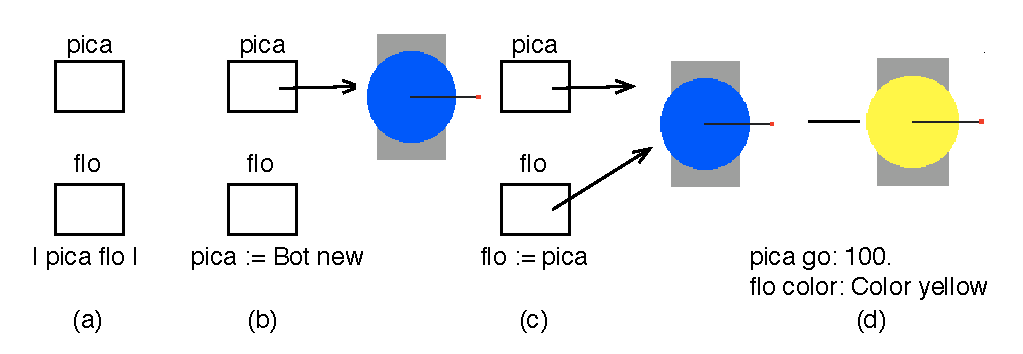
\includegraphics[width=15cm]{boxesPointer}}
\caption{(a) Two variables are declared. (b) A \Turtle is created and the variable \ct{\caro} refers to this new robot. (c) The variable \ct{flo} refers to  to the value of the variable \ct{\caro}, therefore \ct{flo} points to the same object than \ct{\caro}. (d) When we send a message using any of the two variables we actually send a message to the same object.\label{fig:boxesPointerRepresentation}}
\end{center}
\end{figure}


\section{The Right or Left Part of \ct{:=}}
When using a variable name in a script, sometimes it is used to refer to its value as in \ct{size + 100} or \ct{\caro go: 100}. Sometimes it is used to refer to the placeholder
itself to change its value as in \ct{size := 100} or \ct{\caro\ := \Turtle new}. 

The key thing to understand about variables is that using a variable name always refers to the value associated with the variable, except if the variable is \emph{on the left} of an assignment expression \ct{:=}. In this case the variable name represents the placeholder itself and not the variable value. We also say that the value of a variable is always read, except when it appears on the left of \ct{:=} where it is written \ie changed. The script~\ref{scr:placeholder} shows an example. 

\begin{scriptwithouttitle}\label{scr:placeholder}
(1)   | size \caro |		
(2)   \caro := \Turtle new.
(3)   size := 100.	
(4)   size + 100.
(5)   \caro go: size
\end{scriptwithouttitle}

In line 3 of script \ref{scr:placeholder}, the variable name \ct{size} is on the left of \ct{:=}, so it refers to the placeholder. After executing line 3, this variable refers to the number 100.  In line 4, \ct{size + 100} does not participate into an assignment expression so the variable name refers to the variable value. Note that as the result of the addition is not used, this line does not do anything and could be removed. Line 5 both variables \caro and \ct{size} are used to refer to their value \ie object they refer to. Therefore the message \ct{go: 100} is sent to the robot created the line 2.



\largecadre{A variable is a placeholder for a value, an object. Using a variable returns its value except when the variable is on the left of an assignment expression \ct{:=}. In such a case its value changes to become the one of the expression on the right of the assignment expression \ct{:=}. \\
Example. \ct{size + 100} returns 100 added to the value of the variable \ct{size}. \ct{size := 100} changes the value of \ct{size} to be 100.  }




\section{Analyzing Some Simple Scripts}
To  understand better how variables are manipulated, we describe a series of scripts. First read the script and guess what will be result of the script, then evaluate the script and understand its result. We suggest you to draw a box representation when you feel the need and to check with the one we show. The value of a script is normally the value of the last expression that composes it, therefore you can select the script piece by piece and use the \menu{Print It} menu to print the value returned by the script.  As you will see we give a small explanation of script. Note that we do not repeat explanations and  only present the points that are not already covered by the previous explanations. 

\begin{scriptfig}{boxOne}{One}\label{scr:vardeepone}
| \caro size |                
\caro := \Turtle new.
size := 100.     
\caro go: size
\end{scriptfig}

In \scrref{scr:vardeepone}, the variable \caro and \ct{size} are declared. A new robot is created and assigned to the variable \caro. \ct{100} is assigned to the variable \ct{size}. The robot (value assigned to the variable \caro) receives the message \ct{go:} with the value of the variable \ct{size}, here \ct{100} as argument.

\begin{scriptwithouttitle}\label{scr:vardeeptwo}
| \caro size |                
\caro := \Turtle new.
size := 100.	
\caro go: size + 100.
\end{scriptwithouttitle}

In \scrref{scr:vardeeptwo} to find out  to which value the robot should move forward, the expression \ct{size + 100} is calculated. As \ct{size} was initialized with \ct{100} and did not change, the value of \ct{size} is 100, therefore the robot moves forward 200 pixels.
The expression \ct{\caro go: size + 100} in \scrref{scr:vardeeptwo} is equivalent to the expression \ct{\caro go: size2} of \scrref{scr:vardeepthree}. Indeed the variable \ct{size2} has as value the value of the variable \ct{size} plus 100. \ 

\ 

\begin{scriptfig}[0.45]{boxSize2}{with size2}\label{scr:vardeepthree}
| \caro size size2 |                
\caro := \Turtle new.
size := 100.
size2 := size + 100.
\caro go: size2.
\end{scriptfig}

\begin{scriptfig}[0.45]{boxThree}{Changing twice size}\label{scr:vardeepfour}
| \caro size |		
\caro := \Turtle new.
size := 100.	
size := 300.
\caro go: size 
\end{scriptfig}

The value of a variable can indeed change using \ct{:=}. Here, the variable \ct{size} is declared, first we assign \ct{100} to it, then we reassign \ct{300} to it (we dashed the arrow pointing to 100 to stress that the variable takes a new value). 
Therefore when the variable is used its value is 300. As a result the robot moves forward 300 pixels. 


\begin{scriptfig}[.45]{boxNoChange}{Without assignement}\label{src:nouse}
| size \caro |		
\caro := \Turtle new.
size := 100.	
\textbf{size + 200.}
\caro go: size
\end{scriptfig}

The \scriptref{src:nouse} shows that manipulating the value of a variable without reassigning it to a variable does not change its value.  The variable \ct{size} is initialized with \ct{100}. Then the value of size,
here \ct{100}, is added to \ct{200}, but the variable value is not modified. Then \ct{size} value, here \ct{100}, is used to specify how far the robot should move forward. So the robot moves forward 100 pixels.



\begin{scriptfig}[.45]{BoxFour}{Using size to define itself}\label{scr:vardeepfive}
| \caro size |		
\caro := \Turtle new.
size := 100.	
\textbf{size := size + 50.}
\caro go: size
\end{scriptfig}

The variable \ct{size} is initialized to \ct{100}. Then its value is changed to the value of the expression \ct{size + 50}. At this point, \ct{size} value is \ct{100}, so the expression \ct{size + 50} returns \ct{150}. This means that \ct{150} is now assigned to \ct{size}. So the \Turtle moves forward 150 pixels.


\begin{scriptwithouttitle}\label{scr:vardeepten}
| \caro size |		
\caro := \Turtle new.
size := 150.	
\textbf{size := size + size.}
\caro go: size 
\end{scriptwithouttitle}

The variable \ct{size} is initialized to \ct{150}. Then the value of \ct{size} is reassigned to 
refers to the value of the expression \ct{size + size}. When computing the value of the expression \ct{size + size} the value of \ct{size} is 150, therefore the expression returns \ct{300} which is now the new value of the variable \ct{size}. So the robot moves forward 300 pixels.


\summa

\begin{itemize}
\item 
A variable is a placeholder for a value, an object. You can represent a variable as a box referring to an object. 

\item Using a variable returns its value except when the variable is on the left of an assignment expression \ct{:=}. In such a case its value changes to become the one of the expression on the right of the assignment expression \ct{:=}. \\
Example. \ct{size + 100} returns 100 added to the value of the variable \ct{size}. \ct{size := 100} changes the value of \ct{size} to be 100.  
\end{itemize}

\ifx\wholebook\relax\else\end{document}\fi
